\documentclass[tikz,border=6pt]{standalone}
\usepackage{tikz}
\usetikzlibrary{arrows.meta,decorations.pathreplacing}
\definecolor{nebula}{HTML}{6366F1}
\definecolor{spark}{HTML}{14B8A6}
\definecolor{ink}{HTML}{334155}
\begin{document}
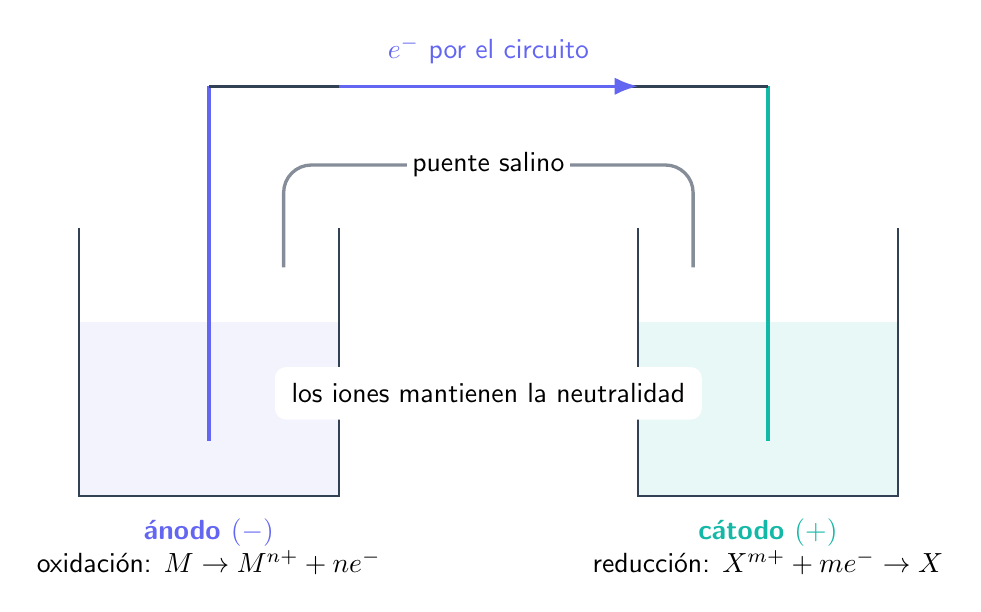
\begin{tikzpicture}[font=\sffamily,>=Latex]
  \fill[nebula!8] (-0.2,0) rectangle (3.1,2.2);
  \fill[spark!10] (6.9,0) rectangle (10.2,2.2);
  \draw[thick,ink] (-0.2,3.4)--(-0.2,0)--(3.1,0)--(3.1,3.4);
  \draw[thick,ink] (6.9,3.4)--(6.9,0)--(10.2,0)--(10.2,3.4);
  \draw[very thick,nebula] (1.45,0.7)--(1.45,5.2);
  \draw[very thick,spark] (8.55,0.7)--(8.55,5.2);
  \draw[very thick,ink] (1.45,5.2)--(8.55,5.2);
  \draw[->,very thick,nebula] (3.1,5.2)--(6.9,5.2) node[midway,above=4pt] {$e^-$ por el circuito};
  \draw[very thick,ink!60,rounded corners=10pt] (2.4,2.9)--(2.4,4.2)--(7.6,4.2)--(7.6,2.9);
  \node[fill=white,inner sep=2pt] at (5,4.2) {puente salino};
  \node[align=center] at (1.45,-0.65) {\textcolor{nebula}{\bfseries \'anodo $(-)$}\\oxidaci\'on: $M\to M^{n+}+ne^-$};
  \node[align=center] at (8.55,-0.65) {\textcolor{spark}{\bfseries c\'atodo $(+)$}\\reducci\'on: $X^{m+}+me^-\to X$};
  \node[fill=white,rounded corners=4pt,inner sep=6pt] at (5,1.3) {los iones mantienen la neutralidad};
\end{tikzpicture}
\end{document}
